%%
%% Author: Dario Chinelli
%% begin 2019-12-04
%% last mod 2022-02-02
%%

% Preamble
\documentclass[class=article, crop=false]{standalone}

% Packages
\usepackage{tikz}
\usetikzlibrary{positioning}

% Document
\begin{document}


\begin{figure}[ht]
\begin{minipage}[c]{0.33\linewidth}
\centering
\resizebox{0.7\textwidth}{!}{%
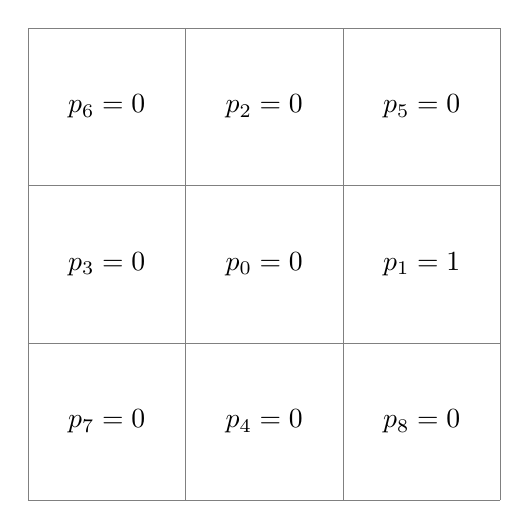
\begin{tikzpicture}
% Lines
\draw[step=2cm, gray, very thin] (0,0) grid (6,6);
% Nodes
\draw (3,3) node[black] {$p_0 = 0$};
\draw (5,3) node[black] {$p_1 = 1$};
\draw (3,5) node[black] {$p_2 = 0$};
\draw (1,3) node[black] {$p_3 = 0$};
\draw (3,1) node[black] {$p_4 = 0$};
\draw (5,5) node[black] {$p_5 = 0$};
\draw (1,5) node[black] {$p_6 = 0$};
\draw (1,1) node[black] {$p_7 = 0$};
\draw (5,1) node[black] {$p_8 = 0$};
\end{tikzpicture}
}%
\captionsetup{width=.8\linewidth}
\caption{First example of probability distribution for a certain position. Always right.}
\label{fig:D2Q9_FirstEx}
\end{minipage}
\begin{minipage}[c]{0.33\linewidth}
\centering
\resizebox{0.7\textwidth}{!}{%
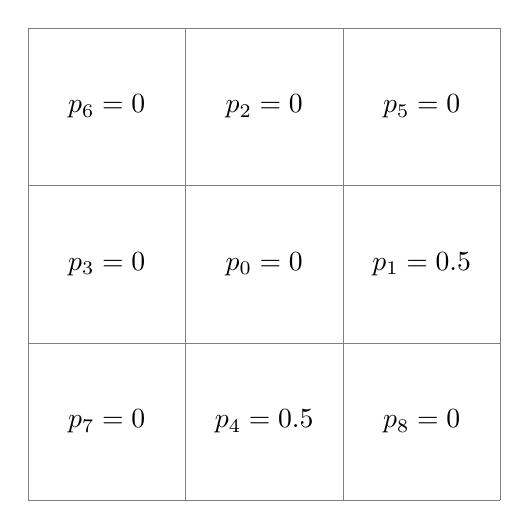
\begin{tikzpicture}
% Lines
\draw[step=2cm, gray, very thin] (0,0) grid (6,6);
% Nodes
\draw (3,3) node[black] {$p_0 = 0$};
\draw (5,3) node[black] {$p_1 = 0.5$};
\draw (3,5) node[black] {$p_2 = 0$};
\draw (1,3) node[black] {$p_3 = 0$};
\draw (3,1) node[black] {$p_4 = 0.5$};
\draw (5,5) node[black] {$p_5 = 0$};
\draw (1,5) node[black] {$p_6 = 0$};
\draw (1,1) node[black] {$p_7 = 0$};
\draw (5,1) node[black] {$p_8 = 0$};
\end{tikzpicture}
}%
\captionsetup{width=.8\linewidth}
\caption{Second example of probability distribution for a certain position. Always right or down.}
\label{fig:D2Q9_SecondEx}
\end{minipage}
\begin{minipage}[c]{0.33\linewidth}
\centering
\resizebox{0.7\textwidth}{!}{%
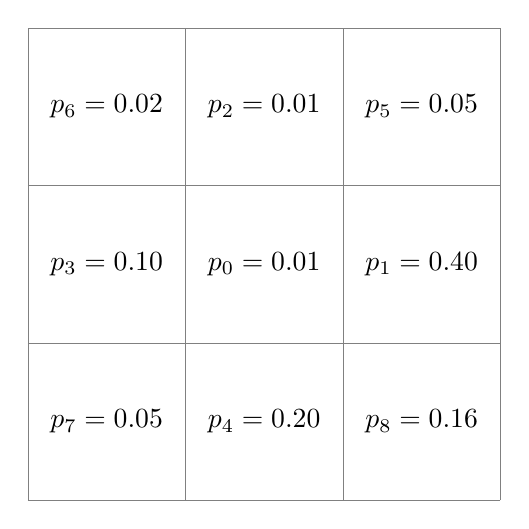
\begin{tikzpicture}
% Lines
\draw[step=2cm, gray, very thin] (0,0) grid (6,6);
% Nodes
\draw (3,3) node[black] {$p_0 = 0.01$};
\draw (5,3) node[black] {$p_1 = 0.40$};
\draw (3,5) node[black] {$p_2 = 0.01$};
\draw (1,3) node[black] {$p_3 = 0.10$};
\draw (3,1) node[black] {$p_4 = 0.20$};
\draw (5,5) node[black] {$p_5 = 0.05$};
\draw (1,5) node[black] {$p_6 = 0.02$};
\draw (1,1) node[black] {$p_7 = 0.05$};
\draw (5,1) node[black] {$p_8 = 0.16$};
\end{tikzpicture}
}%
\captionsetup{width=.8\linewidth}
\caption{Third example of probability distribution for a certain position. None zero probability.}
\label{fig:D2Q9_thirdEx}
\end{minipage}
\end{figure}





\end{document}
